%\documentclass{beamer} %voce pode usar este modelo tambem
\documentclass[t,handout,9pt]{beamer}
\usepackage{graphicx}
\usepackage{url}
\usepackage[british]{babel}
\batchmode
% \pgfpagesuselayout{4 on 1}[letterpaper,landscape,border shrink=5mm]
\usepackage{amsmath}
\usepackage{amssymb}
\usepackage{amsfonts}
\usepackage{enumerate}
\usepackage{epsfig}
\usepackage{bbm}
\usepackage{calc}
\usepackage{adjustbox}
\usepackage{color}
\usepackage{ifthen}
\usepackage{capt-of}
\usepackage{float}
\usepackage{booktabs}
\usepackage{dcolumn}
\usepackage{multicol}
\usepackage{hyperref}
\usepackage[flushleft]{threeparttable}
\usepackage{subcaption}
\usepackage{adjustbox}
\usepackage{ragged2e}
\usepackage{xcolor}
\usepackage{pgfpages}
%\usepackage{showframe}

\usepackage{cmbright}

\renewcommand\ttdefault{cmvtt} % selects CM typewriter

\usepackage[utf8]{inputenc} % Required for inputting international characters
\usepackage[T1]{fontenc} 	% Output font encoding for international characters

%\DeclareFontShape{OT1}{cmss}{b}{n}{<->ssub * cmss/bx/n}{}

\usetheme[compress]{Berlin}
\definecolor{sapienza}{RGB}{0, 49, 83}
\usecolortheme[named=sapienza]{structure}

\usepackage[backend=bibtex,style=alphabetic,giveninits=true,url=false,eprint=false,doi=false]{biblatex}
\DeclareNameAlias{sortname}{last-first}
\renewcommand*{\nameyeardelim}{\addcomma\addspace}
\renewcommand*{\bibfont}{\footnotesize}
\addbibresource{example.bib}
\setbeamerfont{footnote}{size=\tiny}

\setbeamerfont{title}{size=\LARGE}

% reduce spaces between tables/figures and caption
\usepackage[font=small,skip=1pt]{caption}

%% pgf plots stuff
%\usepackage{pgfplots}
%\pgfplotsset{compat=newest}
%% the following commands are needed for some matlab2tikz features
%\usetikzlibrary{plotmarks}
%\usetikzlibrary{arrows.meta}
%\usepgfplotslibrary{patchplots}

% one navigation dot per slide trick
\AtBeginSection[]{\subsection{}}

% fix misbehave for allowframebreaks
\usepackage{etoolbox}
\makeatletter
\patchcmd{\slideentry}{\ifnum#2>0}{\ifnum2>0}{}% replace the subsection number test with a test that always returns true
% use frame numbers instead of subsection slide numbers so that frames broken over slides get separate circles
\patchcmd{\slideentry}{\c@subsectionslide}{\c@framenumber}{}{\@error{unable to patch}}
\patchcmd{\beamer@writeslidentry}{\c@subsectionslide}{\c@framenumber}{}{\@error{unable to patch}}

% date in footer trick
\makeatletter
  \setbeamertemplate{footline}{%
    \begin{beamercolorbox}[colsep=1.5pt]{upper separation line foot}
    \end{beamercolorbox}
    \begin{beamercolorbox}[ht=2.5ex,dp=1.125ex,%
      leftskip=.3cm,rightskip=.3cm plus1fil]{author in head/foot}%
      \leavevmode{\usebeamerfont{author in head/foot}\insertshortauthor}%
      \hfill%
      {\usebeamerfont{institute in head/foot}\usebeamercolor[fg]{institute in head/foot}\insertshortinstitute}%
    \end{beamercolorbox}%
    \begin{beamercolorbox}[ht=2.5ex,dp=1.125ex,%
      leftskip=.3cm,rightskip=.3cm plus1fil]{title in head/foot}%
      {\usebeamerfont{title in head/foot}\insertshorttitle\hfill\insertshortdate}%
    \end{beamercolorbox}%
    \begin{beamercolorbox}[colsep=1.5pt]{lower separation line foot}
    \end{beamercolorbox}
  }
\makeatletter

% remove dot for titlepage and Outline
\makeatletter
\let\old@beamer@writeslidentry\beamer@writeslidentry
\def\beamer@writeslidentry{%
  \expandafter\beamer@ifempty\expandafter{\beamer@framestartpage}{}% does not happen normally
  {%else
    \clearpage\beamer@notesactions%
  }
}
\makeatother

% let's number figure captions
\setbeamertemplate{caption}[numbered]

% trick for grouping equations
\newenvironment{rcases}
  {\left.\begin{aligned}}
  {\end{aligned}\right\rbrace}

%-------------------------Titulo/Autores/Orientador------------------------------------------------
\title[Introduction to Computer Programming]{Introduction to Computer Programming}
\date[A.Y. 2024-2025]{\\A.Y. 2024-2025}
\author[Alessio Martino]{Prof. Alessio Martino\\
\smallskip
{\small \href{mailto:amartino@luiss.it}{\texttt{amartino@luiss.it}}}\\
\smallskip
}
\institute[1/10/2024]{Department of Business and Management\\Viale Romania 32, 00197 Rome\\[\bigskipamount]

\includegraphics[scale=0.4]{Figures/cliente-luiss.png}%
}

%-------------------------Logo na parte de baixo do slide------------------------------------------
%\pgfdeclareimage[height=0.7cm]{senac-logo}{senac-logo.pdf}
%\logo{\pgfuseimage{senac-logo}\hspace*{0.5cm}}

%-------------------------Este código faz o menuzinho bacana na parte superior do slide------------
%\AtBeginSection[]
%{
%  \begin{frame}<beamer>
%    \frametitle{Outline}
%    \tableofcontents[currentsection]
%  \end{frame}
%}
%\beamerdefaultoverlayspecification{<+->}
% -----------------------------------------------------------------------------

\begin{document}
% -----------------------------------------------------------------------------

%---Gerador de Sumário---------------------------------------------------------

\frame[noframenumbering]{
	\titlepage
}

% begin personalization stuff
\setbeamertemplate{navigation symbols}{%
	\insertslidenavigationsymbol
	\insertframenavigationsymbol
	\insertsubsectionnavigationsymbol
	\insertsectionnavigationsymbol
	\insertdocnavigationsymbol
	\insertbackfindforwardnavigationsymbol
	\hspace{1em}%
	\usebeamerfont{footline}
	\insertframenumber/\inserttotalframenumber%
}
\setbeamertemplate{itemize items}[circle]
\setbeamertemplate{enumerate items}[circle]
\setbeamertemplate{bibliography item}{\insertbiblabel}
% end personalization stuff

\section[]{}
%\begin{frame}{Outline}
%	\tableofcontents
%\end{frame}
\begin{frame}{Outline}
\begin{multicols}{2}
  \tableofcontents
\end{multicols}
\end{frame}
%---Fim do Sumário------------------------------------------------------------

% reset navigation dots for other slides
\makeatletter
\let\beamer@writeslidentry\old@beamer@writeslidentry
\makeatother

% -----------------------------------------------------------------------------
\section{Reusing Code}
\begin{frame}{Reusing Code}
\vfill
So far ...
\begin{itemize}
	\item we have covered language mechanisms
	\item we know how to write different \texttt{.py} files for different computations
	\item ... where each file contains some piece of code
	\item ... and each code is a sequence of operations
\end{itemize}
\vfill
\begin{block}{Problem}
This approach is:
\begin{itemize}
	\item easy for small-scale problems
	\item messy for large-scale problems
	\item hard to keep track of details and maintain
	\item hard to reuse inside more complex programs
\end{itemize}
\end{block}
\vfill
\end{frame}
%
\section{Functions}
\begin{frame}{Functions}
\vfill
More code does not necessarily mean good practice $\rightarrow$ use \textcolor{red}{functions}.\\
\vfill
Why?
\begin{itemize}
	\item functions are \textcolor{red}{reusable} chunks of code
	\item functions run if and only if are ``\textcolor{red}{called}'' or ``\textcolor{red}{invoked}''
\end{itemize}
\vfill
Characteristics of a function:
\begin{itemize}
	\item functions have a \textcolor{red}{name}
	\item functions have (0 or more) \textcolor{red}{parameters}
	\item functions have a \textcolor{red}{docstring}\footnote{Optional, but recommended}
	\item functions have a \textcolor{red}{body}
	\item functions return \textcolor{red}{something}.
\end{itemize}
\vfill
\end{frame}
%
\begin{frame}
\begin{figure}
	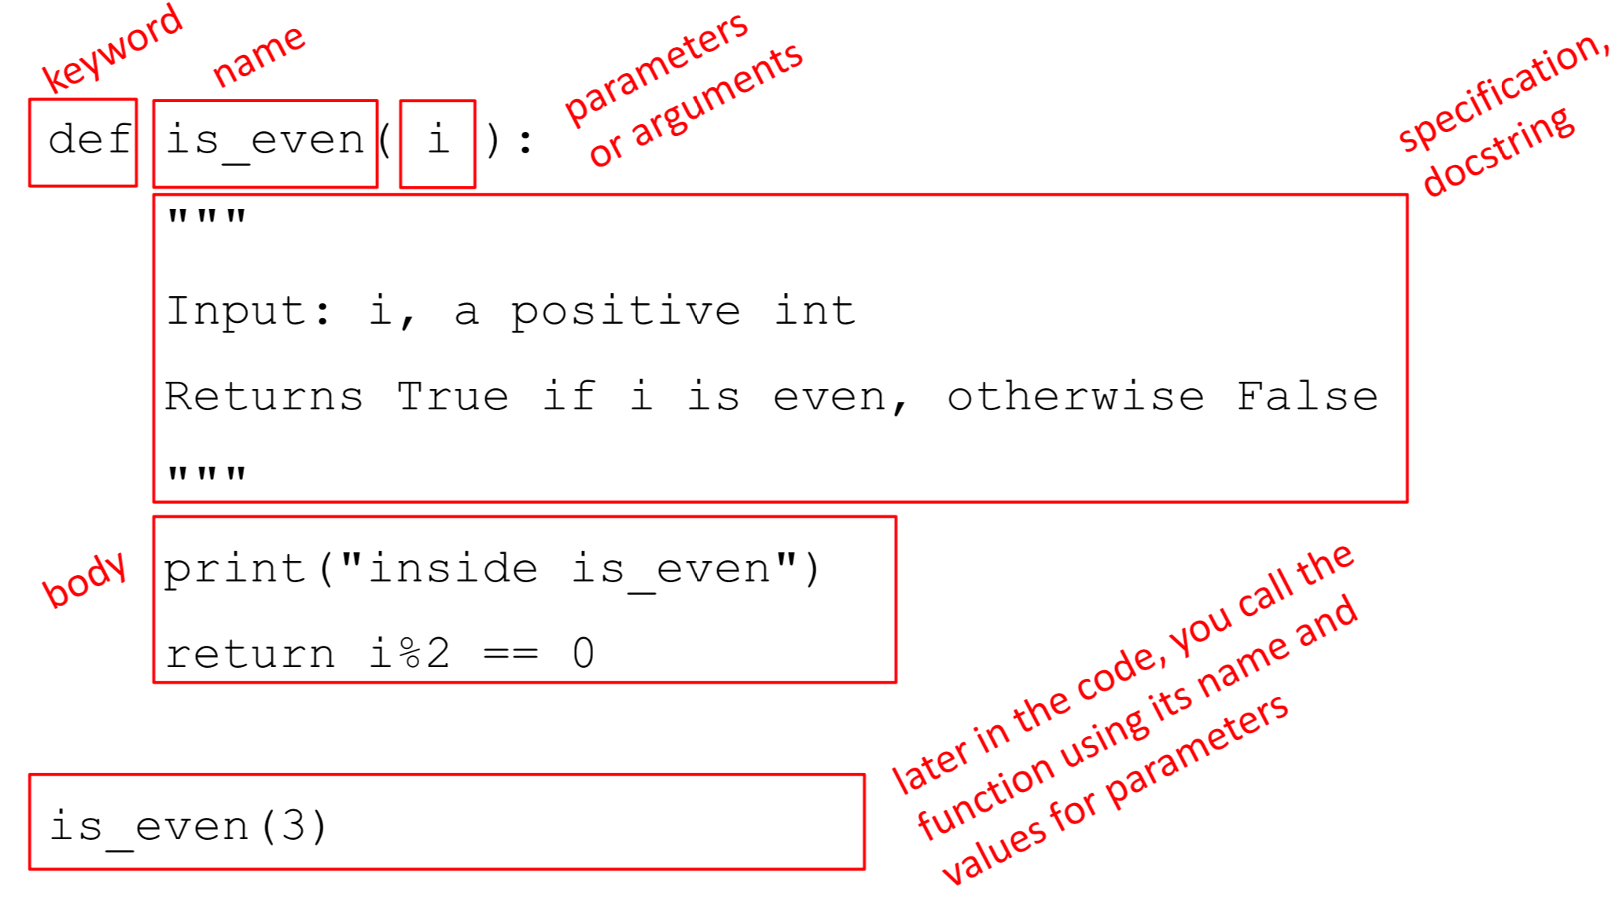
\includegraphics[width=\textwidth]{Figures/Functions}
\caption{Anatomy of a function.}
\end{figure}
\end{frame}
%
\begin{frame}
\begin{figure}
	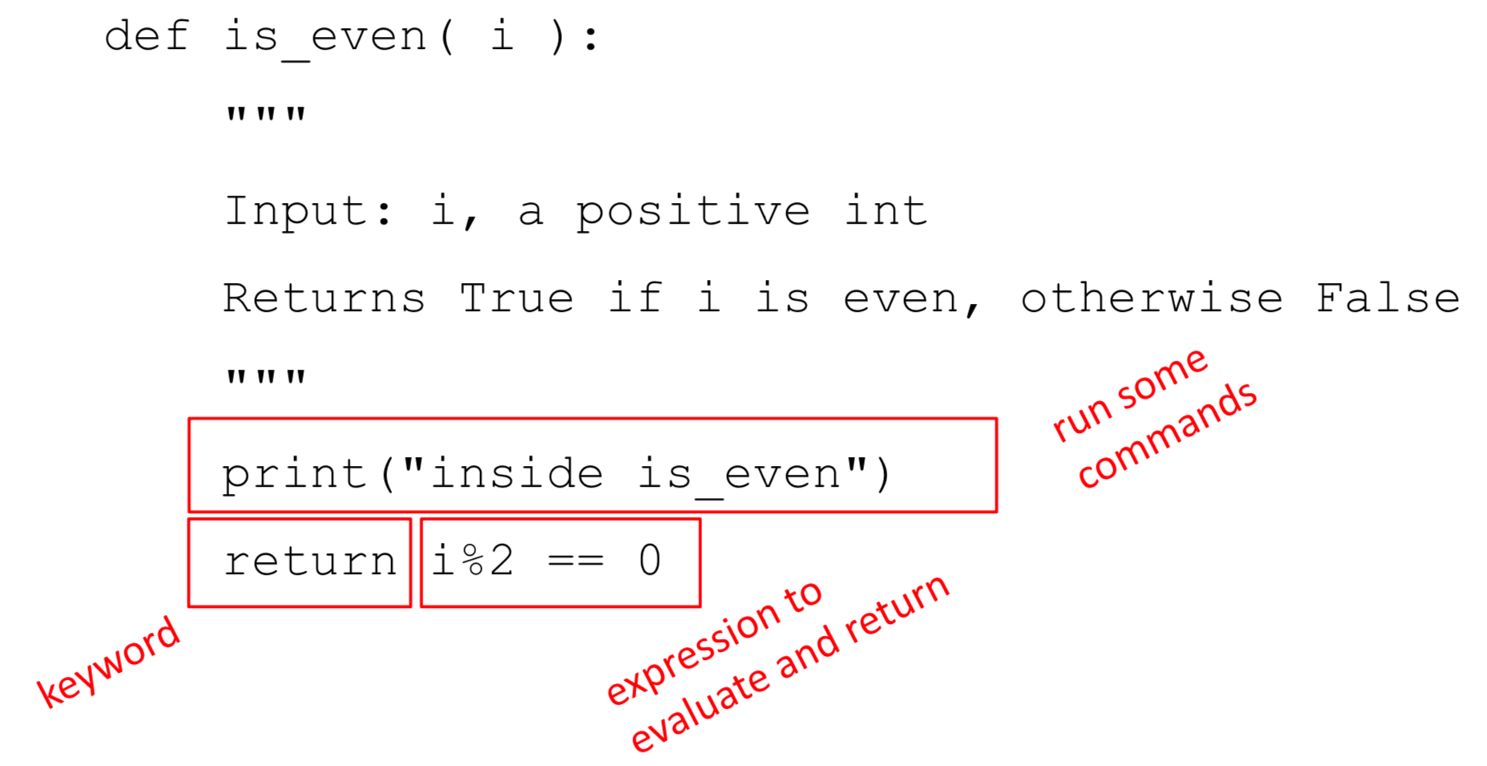
\includegraphics[width=\textwidth]{Figures/Functions2}
\caption{Function body.}
\end{figure}
\end{frame}
%
\begin{frame}
\vfill
\adjustbox{valign=t}{\begin{minipage}[t]{0.49\textwidth}
%\vspace{0.3cm}
When a function is invoked, Python:
\begin{itemize}
	\item creates a \textcolor{red}{frame} for the function call
	\item \textcolor{red}{assigns} arguments to parameters
	\item \textcolor{red}{executes} function body
	\item \textcolor{red}{erases} the frame
\end{itemize}
\end{minipage}}%
\hfill
\adjustbox{valign=t}{\begin{minipage}[t]{0.49\textwidth}
%\vspace{0.3cm}
\begin{table}[]
\begin{flushleft}
\begin{tabular}{ll}
\texttt{def f(i):} &  \\
\texttt{\qquad j = i*2}        & \\
\texttt{\qquad return j}        & \\
\texttt{\qquad }        & \\
\texttt{n=f(1)}        & \\
\texttt{n=f(2)}        & \\
\texttt{n=f(3)}        & \\
\end{tabular}
\end{flushleft}
\end{table}
\end{minipage}}
\vfill
Let's see it in Python Tutor\\
\quad \url{http://pythontutor.com/}
\vfill
\end{frame}
%
\begin{frame}
\vfill
The importance of \texttt{return}:
\begin{figure}
	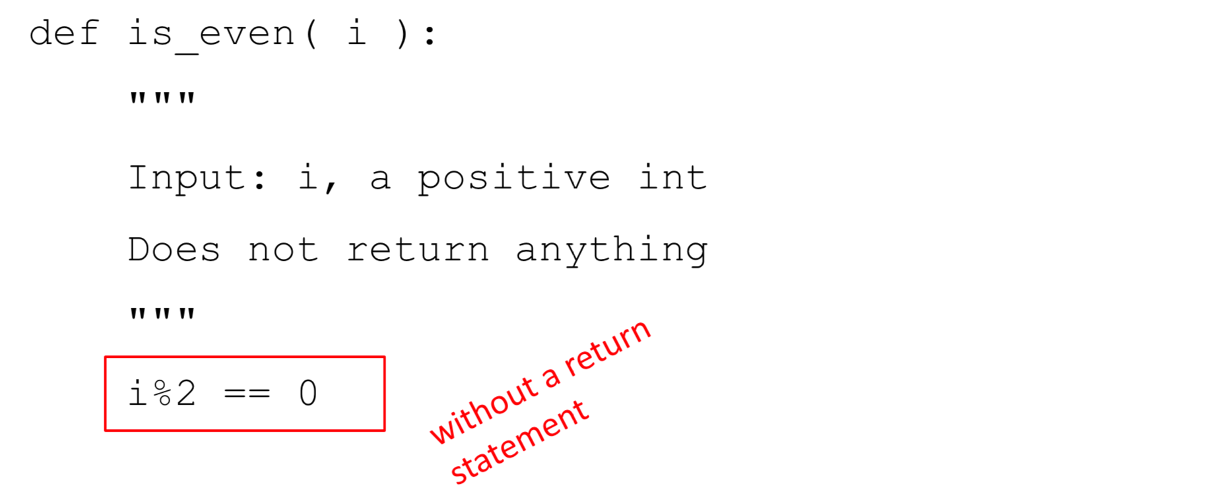
\includegraphics[width=\textwidth]{Figures/Functions3}
%\caption{Function body.}
\end{figure}
\vfill
What happens when running e.g.
\begin{table}[]
\begin{flushleft}
\begin{tabular}{ll}
\texttt{n=is\_even(2)}        & \\
\end{tabular}
\end{flushleft}
\end{table}
\begin{itemize}
	\item Python returns \texttt{None} if no \texttt{return} is given
	\item \texttt{None} represents the absence of a value
\end{itemize}
\vfill
\end{frame}
%
\subsection{\texttt{print} vs. \texttt{return}}
\begin{frame}
\vfill
\adjustbox{valign=t}{\begin{minipage}[t]{0.49\textwidth}
%\vspace{0.3cm}
\texttt{print}
\begin{itemize}
	\item can be placed \textcolor{red}{anywhere} (inside and/or outside functions)
	\item as \textcolor{red}{many} \texttt{print} statements as you want
	\item code \textcolor{red}{after} \texttt{print} statements is executed inside a function
	\item has a value associated to it, \textcolor{red}{outputted} to the console
\end{itemize}
\end{minipage}}%
\hfill
\adjustbox{valign=t}{\begin{minipage}[t]{0.49\textwidth}
%\vspace{0.3cm}
\texttt{return}
\begin{itemize}
	\item has a meaning only \textcolor{red}{inside} a function
	\item only \textcolor{red}{one} \texttt{return} statement inside a function
	\item code \textcolor{red}{after} \texttt{return} statement is not executed
	\item has a value associated to it, \textcolor{red}{returned} to the function caller
\end{itemize}
\end{minipage}}
\vfill
\end{frame}
%
\subsection{One return, multiple values}
\begin{frame}
The \texttt{return} statement can return multiple values (if needed):
\begin{itemize}
	\item list of values separated by commas
	\item returns a tuple\footnote{We will see tuples later in the course, for now we just print multiple outputs.}
\end{itemize}
\vfill
Example:
\vspace{-0.4cm}
\begin{table}[]
\begin{flushleft}
\begin{tabular}{ll}
\texttt{def hms(nsec):}        & \\
\texttt{\quad """Takes nsec (n. of seconds) and splits in hours, minutes, seconds"""}        & \\
\texttt{\quad hh = nsec // 3600}        & \\
\texttt{\quad nsec = nsec \% 3600}        & \\
\texttt{\quad mm = nsec // 60}        & \\
\texttt{\quad ss = nsec \% 60}        & \\
\texttt{\quad return hh, mm, ss}        & \\
\texttt{\quad}        & \\
\texttt{print(hms(4000))}        & \\
\texttt{\# Out: (1, 6, 40)}        & \\
\texttt{print(hms(100000))}        & \\
\texttt{\# Out: (27, 46, 40)}        & \\
\end{tabular}
\end{flushleft}
\end{table}
\end{frame}
%
\section{Variable Scope}
\begin{frame}{Variable Scope}
\begin{figure}
	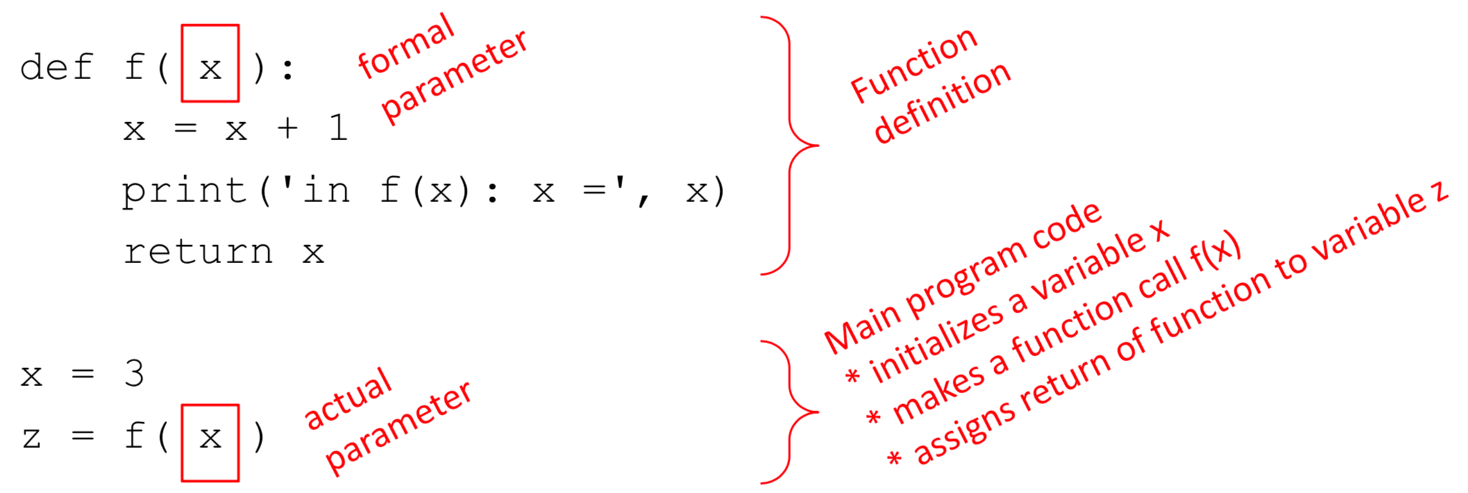
\includegraphics[width=\textwidth]{Figures/Scope1}
\caption{Variable scope (inside/outside function).}
\end{figure}
\begin{itemize}
	\item the \textcolor{red}{formal parameter} gets bound to the \textcolor{red}{actual parameter} when the function is called
	\item when entering a function, a new \textcolor{red}{scope} (or \textcolor{red}{frame}, or \textcolor{red}{environment}) is created
	\item the \textcolor{red}{scope} is the mapping of names to objects
\end{itemize}
\end{frame}
%
\subsection{Running Example}
\begin{frame}
\vfill
\begin{figure}
	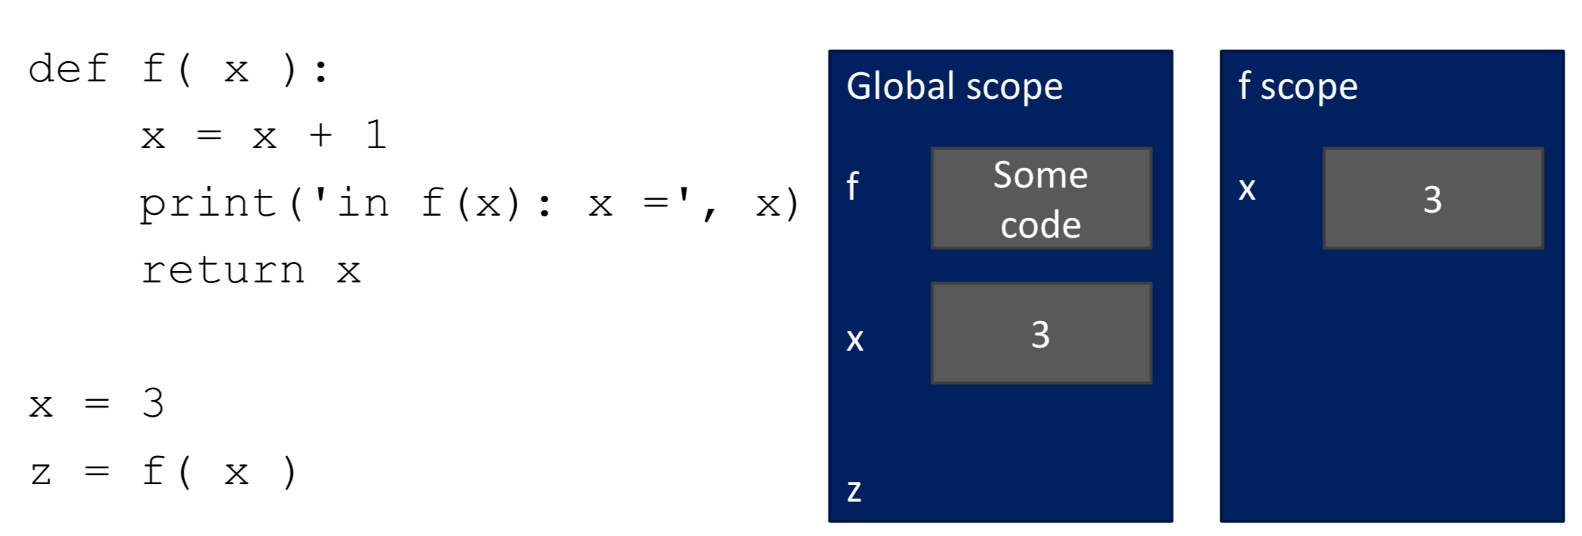
\includegraphics[width=\textwidth]{Figures/Example1}
\caption{Step 1 of 4.}
\end{figure}
\vfill
What's going on here?
\begin{enumerate}
	\item in the main (i.e., global) scope, we define function \texttt{f}
	\item in the main scope, we define variable \texttt{x}
	\item function \texttt{f} is called and variable \texttt{x} is fed to \texttt{f}
\end{enumerate}
\vfill
\end{frame}
%
\begin{frame}
\vfill
\begin{figure}
	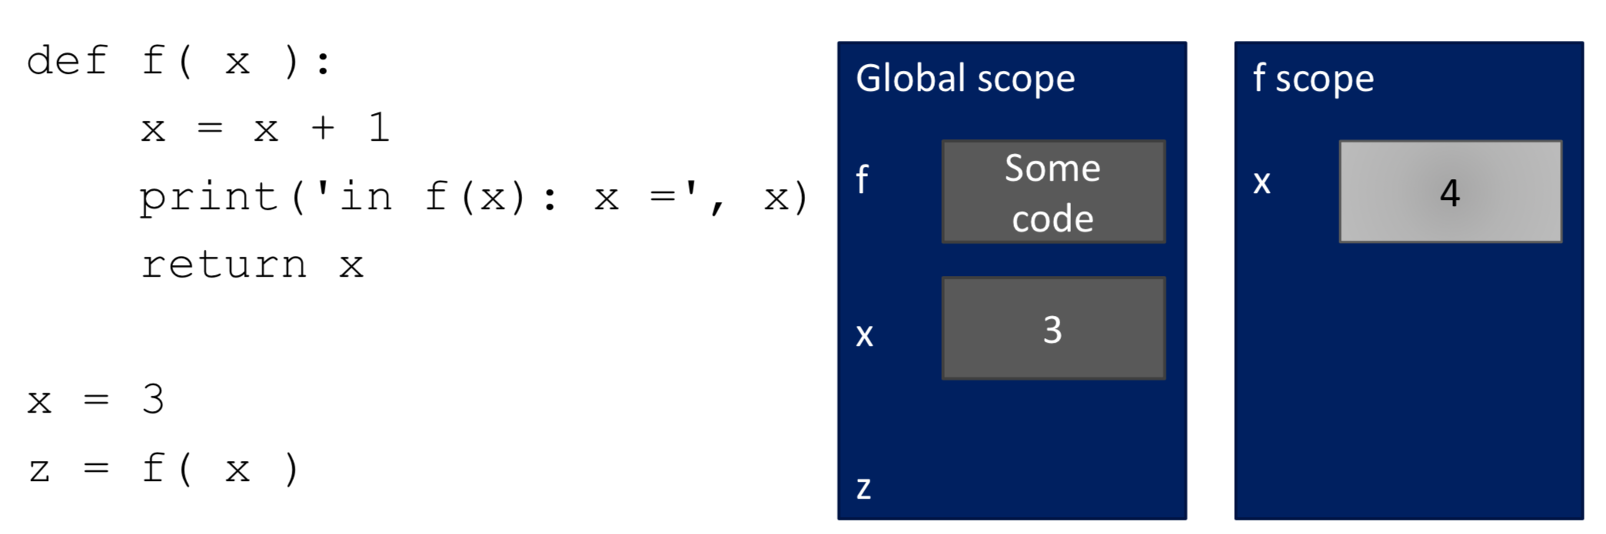
\includegraphics[width=\textwidth]{Figures/Example2}
\caption{Step 2 of 4.}
\end{figure}
\vfill
What's going on here?
\begin{enumerate}
	\item variable \texttt{x} is changed inside \texttt{f} because of \texttt{x = x+1}
\end{enumerate}
\begin{block}{Note}
Variable \texttt{x} in the global scope has not been changed because \texttt{f} has its own scope!
\end{block}
\vfill
\end{frame}
%
\begin{frame}
\vfill
\begin{figure}
	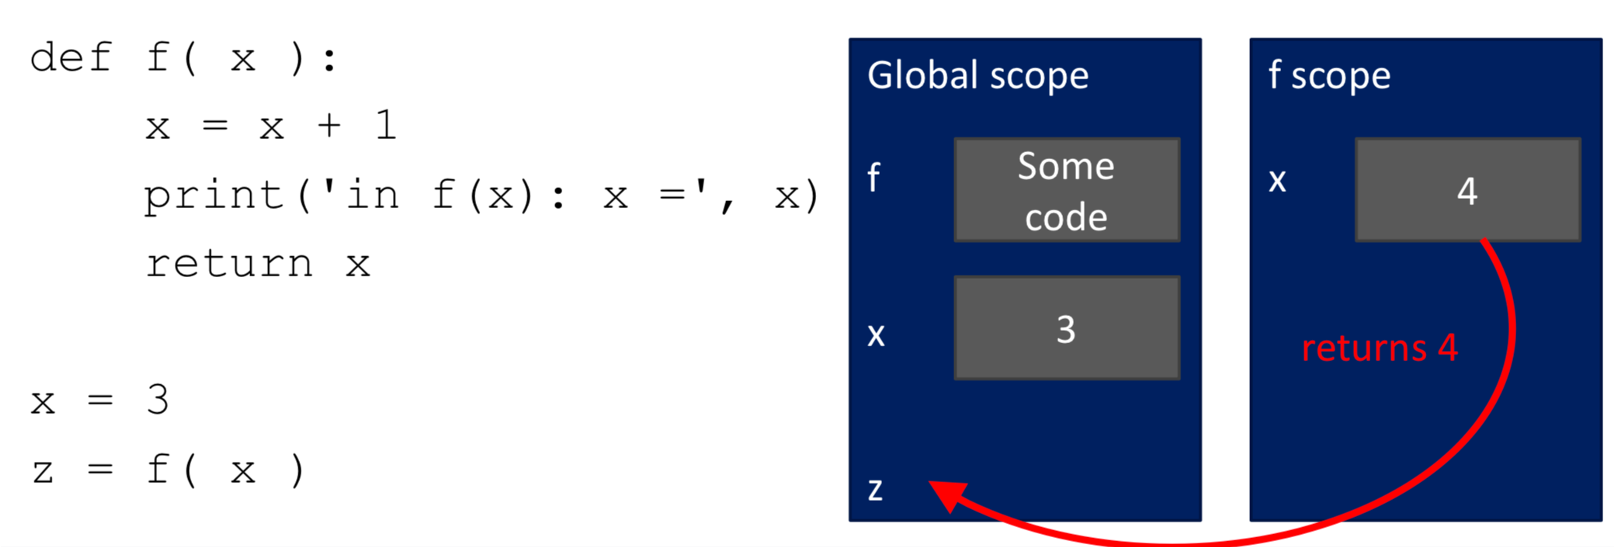
\includegraphics[width=\textwidth]{Figures/Example3}
\caption{Step 3 of 4.}
\end{figure}
\vfill
What's going on here?
\begin{enumerate}
	\item variable \texttt{x} inside \texttt{f} is ready to be \texttt{return}ed
	\item in the main scope, there is variable \texttt{z} ready to host the \texttt{return}ed value
\end{enumerate}
\vfill
\end{frame}
%
\begin{frame}
\vfill
\begin{figure}
	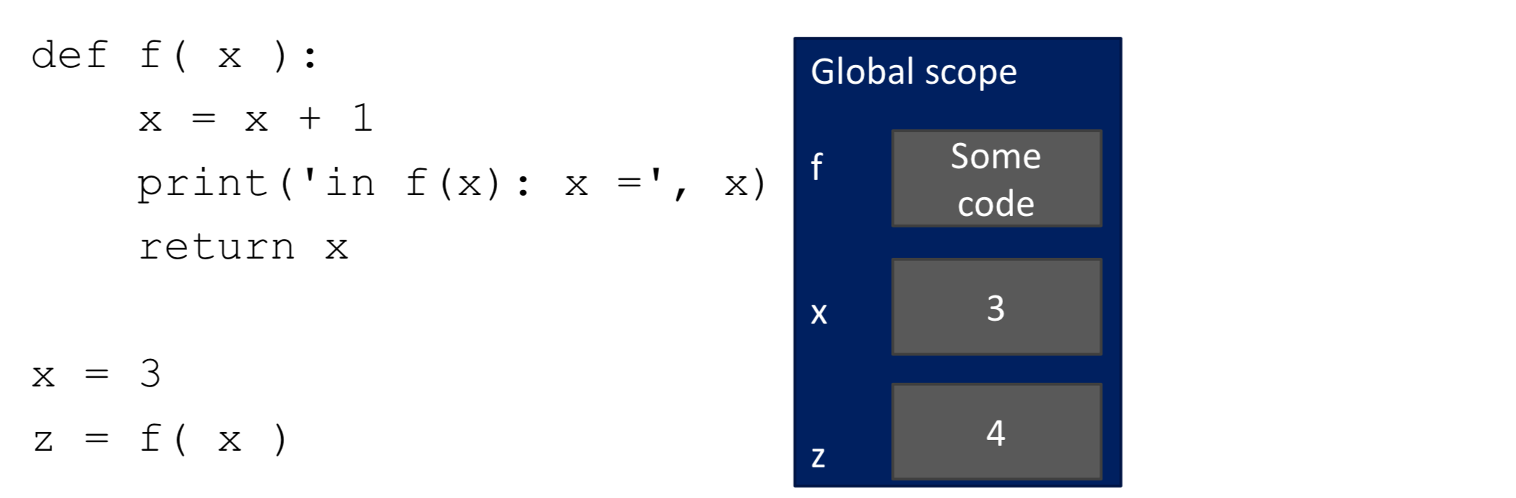
\includegraphics[width=\textwidth]{Figures/Example4}
\caption{Step 4 of 4.}
\end{figure}
\vfill
What's going on here?
\begin{enumerate}
	\item the frame of function \texttt{f} is destroyed because its execution is finished
	\item in the main scope, we have the `original' value for \texttt{x}
	\item in the main scope, we have the output of function \texttt{f} in the new variable \texttt{z}
\end{enumerate}
\vfill
\end{frame}
%
\subsection{Important Caveats on Variable Scopes}
\begin{frame}
\vfill
\begin{figure}
	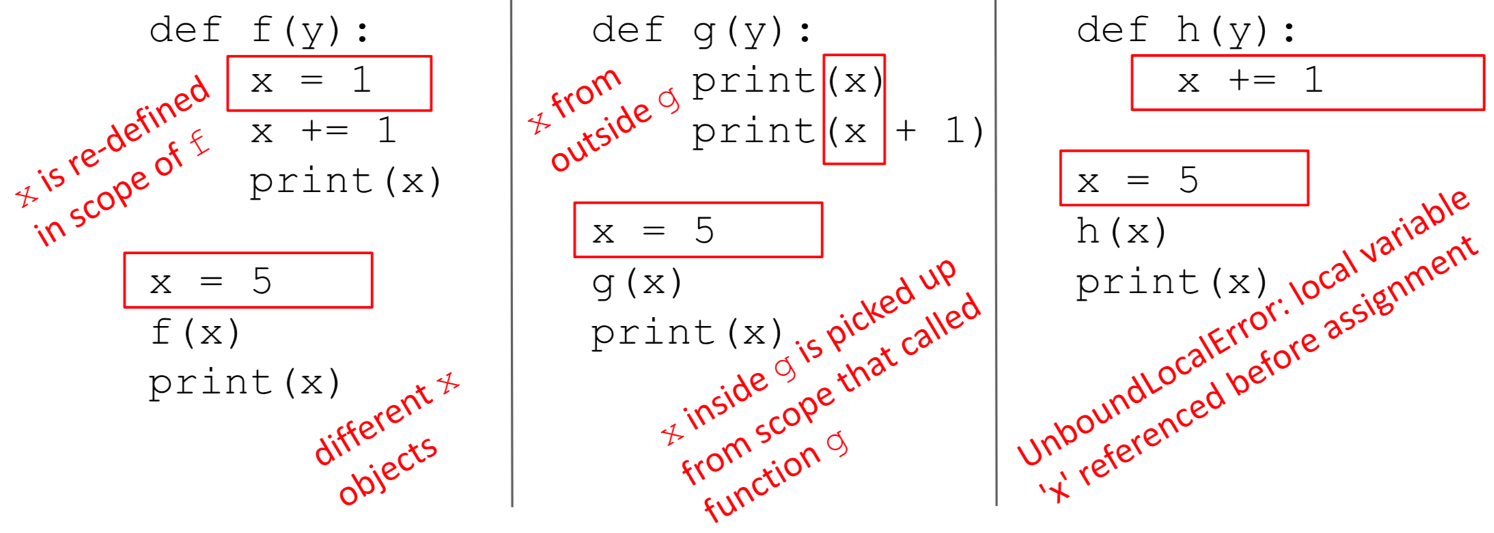
\includegraphics[width=\textwidth]{Figures/Scope2}
\caption{Important caveats (pt.1).}
\end{figure}
\vfill
\begin{itemize}
	\item inside a function, you \textcolor{red}{can access} variables defined outside the function itself
	\item inside a function, you \textcolor{red}{cannot modify} variables defined outside the function itself
	\item to modify variables defined outside, you must use the \texttt{global} keyword ... which is frowned upon
\end{itemize}
\vfill
\end{frame}
%
\begin{frame}
\vfill
\begin{figure}
	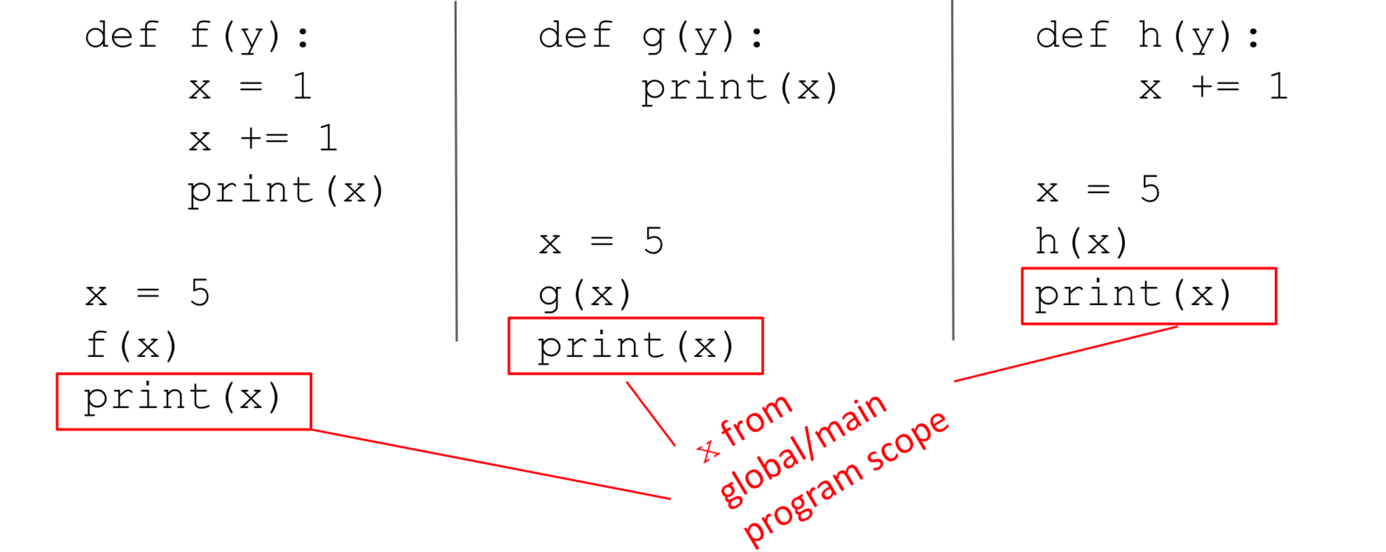
\includegraphics[width=\textwidth]{Figures/Scope3}
\caption{Important caveats (pt.2).}
\end{figure}
\vfill
\begin{itemize}
	\item due to the fact that (by default) you cannot modify variables inside a function, \texttt{x} remains untouched
\end{itemize}
\vfill
\end{frame}
%
\subsection{The \texttt{global} Keyword}
\begin{frame}
\vfill
\adjustbox{valign=t}{\begin{minipage}[t]{0.49\textwidth}
%\vspace{0.3cm}
\begin{itemize}
	\item when we create a variable \textcolor{red}{inside} a function, it is \textcolor{red}{local} by default
	\item when we create a variable \textcolor{red}{outside} a function, it is \textcolor{red}{global} by default: no need to use the \texttt{global} keyword
	\item using the \texttt{global} keyword outside a function has no effect
	\item we use the \texttt{global} keyword to \textit{write}/\textit{modify} a variable \textcolor{red}{inside} a function
\end{itemize}
\end{minipage}}%
\hfill
\adjustbox{valign=t}{\begin{minipage}[t]{0.49\textwidth}
%\vspace{0.3cm}
\begin{table}[]
\begin{flushleft}
\begin{tabular}{ll}
\texttt{c=0 \# global variable}        & \\
\texttt{\quad }        & \\
\texttt{def add():}        & \\
\texttt{\quad global c}        & \\
\texttt{\quad c = c + 2 \# increment by 2}        & \\
\texttt{\quad print("Inside add(): c = ", c)}        & \\
\texttt{\quad }        & \\
\texttt{add()}        & \\
\texttt{print("In main(): c = ", c)}        & \\
\end{tabular}
\end{flushleft}
\end{table}
\end{minipage}}
\vfill
\end{frame}
%
\subsection{Nested Functions}
\begin{frame}
\vfill
\adjustbox{valign=t}{\begin{minipage}[t]{0.49\textwidth}
%\vspace{0.3cm}
\begin{itemize}
	\item you can \textcolor{red}{nest} functions arbitrarily
	\item scopes of nested functions behave like Matryoshka dolls
	\item let's see how thanks to PythonTutor\\
	\quad \url{http://pythontutor.com/}
\end{itemize}
\end{minipage}}%
\hfill
\adjustbox{valign=t}{\begin{minipage}[t]{0.49\textwidth}
%\vspace{0.3cm}
\begin{table}[]
\begin{flushleft}
\begin{tabular}{ll}
\texttt{def g(x):}        & \\
\texttt{\quad def h():}        & \\
\texttt{\quad\quad x = 'abc'}        & \\
\texttt{\quad x = x + 1}        & \\
\texttt{\quad print('g: x =', x)}        & \\
\texttt{\quad h()}        & \\
\texttt{\quad return x}        & \\
\texttt{\quad }        & \\
\texttt{x = 3}        & \\
\texttt{z = g(x)}        & \\
\end{tabular}
\end{flushleft}
\end{table}
\end{minipage}}
\vfill
\end{frame}
%
\section{Positional vs. Keyword Arguments}
\begin{frame}{Positional vs. Keyword Arguments}
We have seen \textcolor{red}{positional bounding} of formal parameters to actual parameters:
\begin{itemize}
	\item the first formal parameter is bound to the first actual parameter
	\item the second formal to the second actual
	\item ... and so on, until all parameters are bounded
\end{itemize}
Python also supports \textcolor{red}{keyword bounding}
\begin{itemize}
	\item formals are bound to actuals using the name of the formal parameter
\end{itemize}
Example:
\begin{table}[]
\begin{flushleft}
\begin{tabular}{ll}
\texttt{def add(a, b, c):}        & \\
\texttt{\quad return a + b + c}        & \\
\texttt{\quad}        & \\
\texttt{add(1,2,3)}        & \# positional bounding \texttt{a$\rightarrow$1}, \texttt{b$\rightarrow$2}, \texttt{c$\rightarrow$3}\\
\texttt{add(c=3, a=1, b=2)}        & \# keyword bounding (order does not matter)\\
\end{tabular}
\end{flushleft}
\end{table}
\end{frame}
%
\subsection{Optional and Default Parameters}
\begin{frame}
\textcolor{red}{All} parameters need to be provided to a function:
\begin{itemize}
	\item via positional or keyword arguments
	\item via default parameters
\end{itemize}
Example:
\begin{table}[]
\begin{flushleft}
\begin{tabular}{ll}
\texttt{def area\_cylinder(radius=1, height=1):}        & \\
\texttt{\quad pi = 3.14}        & \\
\texttt{\quad bottom\_area = pi * radius ** 2}        & \\
\texttt{\quad side\_area = pi * height * radius * 2}        & \\
\texttt{\quad return side\_area + bottom\_area * 2}        & \\
\texttt{\quad}        & \\
\texttt{print("No parameters: ", area\_cylinder(), "$\backslash$n")}        & \\
\texttt{\quad}        & \\
\texttt{print("One parameter: ", area\_cylinder(2))}        & \\
\texttt{print("Check: ", area\_cylinder(2, 1), "$\backslash$n")}        & \\
\texttt{\quad}        & \\
\texttt{print("Two parameters: ", area\_cylinder(2, 3), "$\backslash$n")}        & \\
\texttt{\quad}        & \\
\texttt{print("Specific parameters: ", area\_cylinder(height=2))}        & \\
\texttt{print("Check: ", area\_cylinder(1, 2), "$\backslash$n")}        & \\
\end{tabular}
\end{flushleft}
\end{table}
\end{frame}
%
\section{Built-in Functions}
\begin{frame}{Built-in Functions}
\vfill
Python implements many functions by default, which are called \textcolor{red}{built-in functions}.
\vfill
Examples of built-in functions:
\begin{itemize}
	\item numerical functions, such as \texttt{round(x)} and \texttt{pow(x,y)}\footnote{Which is another way of doing exponentiation: \texttt{pow(x,y)} is the same as \texttt{x**y}.}
	\item casting, such as \texttt{int(x)}, \texttt{float(x)} and \texttt{str(x)}
	\item input and output, namely \texttt{input()} and \texttt{print()}
	\item help function, namely \texttt{help()}\footnote{The \texttt{help()} function takes as input the name of a function and returns its docstring.}
\end{itemize}
\vfill
Related functions are grouped into files, called \textcolor{red}{modules}.
\vfill
\end{frame}
%
\section{Modules}
\begin{frame}{Modules}
\vfill
\textcolor{red}{Modular programming} is the way of breaking a large, unwieldy programming task into separate, smaller (and more manageable) subtasks.
\vfill
A \textcolor{red}{module} is a piece of software with a specific functionality.\\
For example, a game (e.g., chess, ping-pong, ...):
\begin{itemize}
	\item a module responsible for the game logic (rules)
	\item a module responsible for graphics
\end{itemize}
\vfill
In Python, each module is a Python file with a \texttt{.py} extension, yet other extensions are also possible (e.g., pre-compiled \texttt{C++}).
\vfill
Modules contain some Python code (e.g., functions, class definitions, ...).
\vfill
\end{frame}
%
\begin{frame}
An example: the \texttt{random} module.
\begin{center}\texttt{random.py}\end{center}
\begin{table}[]
\begin{flushleft}
\begin{tabular}{ll}
\texttt{def sample(...):}        & \\
\texttt{\quad """Chooses k unique random elements from a population..."""}        & \\
\texttt{\quad some code}        & \\
\texttt{\quad some code}        & \\
\texttt{\quad}        & \\
\texttt{def randint(...):}        & \\
\texttt{\quad """Return random integer in range [a, b], including both end points."""}        & \\
\texttt{\quad some code}        & \\
\texttt{\quad some code}        & \\
\texttt{\quad}        & \\
\texttt{def random(...):}        & \\
\texttt{\quad """Get the next random number in the range [0.0, 1.0)."""}        & \\
\texttt{\quad some code}        & \\
\texttt{\quad some code}        & \\
\end{tabular}
\end{flushleft}
\end{table}
\end{frame}
%
\subsection{Using Modules in Python}
\begin{frame}
Modules are \textcolor{red}{imported} (in your script, in your function or in other modules) using the \texttt{import} command.
\vfill
You can use two different strategies for using a specific function from that module.
\begin{enumerate}
	\item using the \texttt{<module>.<function>} notation\\
	\begin{table}[]
	\begin{flushleft}
	\begin{tabular}{ll}
	\texttt{>{}>{}> import random}        & $\rightarrow$ or any other module\\
	\texttt{>{}>{}> print(random.randint(1, 100))}        & $\rightarrow$ or any other function\\
	\texttt{65}        & $\rightarrow$ your result might vary\\
	\end{tabular}
	\end{flushleft}
	\end{table}
	\item using the \texttt{from} command\\
	\begin{table}[]
	\begin{flushleft}
	\begin{tabular}{ll}
	\texttt{>{}>{}> from random import randint}        & $\rightarrow$ or any other function\\
	\texttt{>{}>{}> print(randint(1, 100))}        &  \\
	\texttt{65}        & $\rightarrow$ your result might vary\\
	\end{tabular}
	\end{flushleft}
	\end{table}
\end{enumerate}
\vfill
\begin{block}{Warning}
Strategy \#2 does not need the dot-notation (see Strategy \#1). Yet, it only loads a specific function in your main!
\end{block}
\vfill
\end{frame}
%
\subsection{Common Modules in Python}
\begin{frame}
Python comes with many modules, including:
\vfill
\begin{description}
	\item[\texttt{io}] read and write from files
	\item[\texttt{math}] mathematical functions
	\item[\texttt{random}] pseudo-random number generator
	\item[\texttt{string}] useful string functions
	\item[\texttt{sys}] information about your operating system
\end{description}
\vfill
You can find the full list here:
\begin{center}
	\url{https://docs.python.org/3/library/}
\end{center}
\vfill
\end{frame}
%
\begin{frame}
An example: the \texttt{math} module:
\begin{itemize}
	\item Number-theoretic and representation functions
	\item Power and logarithmic functions
	\item Trigonometric functions
	\item Angular conversion
	\item Hyperbolic functions
	\item Special functions and constants
\end{itemize}
\begin{table}[]
\begin{flushleft}
\begin{tabular}{ll}
\texttt{>{}>{}> import math}        & \\
\texttt{>{}>{}> print(math.factorial(x))}        & \# return $x!$\\
\texttt{>{}>{}> print(math.log2(x))}        & \# return the base-2 logarithm of $x$\\
\texttt{>{}>{}> print(math.cos(math.pi))}        & \# return the cosine of $\pi$\\
\texttt{>{}>{}> print(math.gcd(x,y))}        & \# return the greatest common divisor\\
\end{tabular}
\end{flushleft}
\end{table}
\vfill
You can find the full list here:
\begin{center}
	\url{https://docs.python.org/3/library/math.html}
\end{center}
\vfill
\end{frame}
%
\subsection{Interactive Documentation}
\begin{frame}
You can browse the contents of a module interactively via the \texttt{dir()} function.
\vfill
\begin{table}[]
\begin{flushleft}
\begin{tabular}{ll}
\texttt{>{}>{}> import math}        & \\
\texttt{>{}>{}> print(dir(math))}        & \\
\texttt{['\_\_doc\_\_', '\_\_file\_\_', '\_\_loader\_\_', '\_\_name\_\_', '\_\_package\_\_',}        &\\
\texttt{'\_\_spec\_\_', 'acos', 'acosh', 'asin', 'asinh', 'atan', 'atan2', 'atanh', 'ceil',}        &\\
\texttt{'comb', 'copysign', 'cos', 'cosh', 'degrees', 'dist', 'e', 'erf', 'erfc', 'exp', 'expm1',}        &\\
\texttt{'fabs', 'factorial', 'floor', 'fmod', 'frexp', 'fsum','gamma', 'gcd', 'hypot',}        &\\
\texttt{'inf', 'isclose', 'isfinite', 'isinf', 'isnan', 'isqrt', 'lcm', 'ldexp', 'lgamma',}        &\\
\texttt{'log', 'log10', 'log1p', 'log2', 'modf', 'nan', 'nextafter', 'perm', 'pi', 'pow',}        &\\
\texttt{'prod', 'radians', 'remainder', 'sin', 'sinh', 'sqrt', 'tan', 'tanh',}        &\\
\texttt{'tau', 'trunc', 'ulp']}        &\\
\end{tabular}
\end{flushleft}
\end{table}
\vfill
\begin{block}{Note}
Items beginning/ending with \texttt{'\_\_'} are some metadata files. You can safely ignore them. For example, \texttt{'\_\_file\_\_'} contains the path pointing to the module source file.
\end{block}
\vfill
\end{frame}
%
\begin{frame}
Given a list of functions, you can browse their documentation via the \texttt{help()} function.
\begin{block}{Recall}
The \texttt{help()} function takes as input the name of a function and returns its docstring.
\end{block}
\vfill
\begin{table}[]
\begin{flushleft}
\begin{tabular}{ll}
\texttt{>{}>{}> import math}        & \\
\texttt{>{}>{}> help(math.log)}        & \\
\texttt{Help on built-in function log in module math:}        &\\
\texttt{\quad}        &\\
\texttt{log(...)}        &\\
\texttt{\quad}        &\\
\texttt{\quad log(x, [base=math.e])}        &\\
\texttt{\quad If the base not specified, returns the natural logarithm (base e) of x.}        &\\
\texttt{\quad}  &\\
\texttt{(END)}  &\\
\end{tabular}
\end{flushleft}
\end{table}
\vfill
%\begin{block}{Note}
%The \texttt{help()} function works also with your own functions, if you provide a docstring.
%\end{block}
%\vfill
\end{frame}
%------------------------------------------------------------------------------
%\section{References}
%\begin{frame}[allowframebreaks]{References}
%%\bibliographystyle{apacite}
%\printbibliography[heading=none]
%\end{frame}
\section{References}
\begin{frame}{References}
\begin{itemize}
	\item Guttag, J. V. (2013). \textit{Introduction to Computation and Programming using Python (Revised and Expanded Edition)}. MIT Press. [Chapter 4]
	\item Downey, A. (2015). \textit{Think Python}. Green Tea Press ed. 2nd. [Chapter 3]
\end{itemize}
\end{frame}
%------------------------------------------------------------------------------
\section{Acknowledgments}
\begin{frame}{Acknowledgments}
% \begin{itemize}
% 	\item Prof. Irene Finocchi (LUISS University)\\
% 	\quad \textit{Introduction to Computer Programming} Lecture Notes (2020-2021)
% \end{itemize}
\end{frame}
%------------------------------------------------------------------------------
%\subsection{Sites legais}
%\begin{frame}{Sites legais}
%  Want to know more? See!
%  \begin{itemize}
%    \item Browse in my page \url{http://www.ezefranca.com}.
%    \item Browse on BCC page \url{http://www.sp.senac.br/bcc}.
%    \item Thanks WriteLaTeX from Support! \url{http://www.writelatex.com}.
%  \end{itemize}
%
%\end{frame}
%------------------------------------------------------------------------------

% -----------------------------------------------------------------------------
\end{document}
%-----------------------------------------------Este comentario nunca aparecera
